\documentclass{article}
\usepackage[dvipsnames]{xcolor}
\usepackage{cantoneseornament}
\usepackage{sinoglyph}

\begin{document}

\section{Single ornaments}
\cantoneseornament[width=2cm, color=SeaGreen]{1}\quad
\cantoneseornament[width=2cm, color=Maroon]{51}\quad
\cantoneseornament[width=2cm, color=MidnightBlue]{76}

\section{Symmetry}
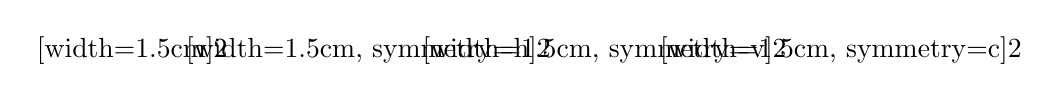
\begin{tikzpicture}
  \node at (0,0) {\cantoneseornament[width=1.5cm]{2}};
  \node at (3,0) {\cantoneseornament[width=1.5cm, symmetry=h]{2}};
  \node at (6,0) {\cantoneseornament[width=1.5cm, symmetry=v]{2}};
  \node at (9,0) {\cantoneseornament[width=1.5cm, symmetry=c]{2}};
\end{tikzpicture}

\section{Frame}
\begin{center}
  \cantoneseframe[corner=1, edge=16, width=6cm, height=4cm, color=Maroon]{%
    \centering Cantonese frame test}
\end{center}

\section{Divider}
\cantonesedivider[width=10cm, ornament width=1.5cm]{4}

\section{Frame presets}
\begin{center}
  \cantoneseframepreset{lingnan}
  \cantoneseframe[width=5cm, height=3cm]{Lingnan preset}
\end{center}

\section{Sinoglyph prototype}
\sinoglyphborder[repeat=6]{門}

\end{document}
